\chapter{Estat de l'art}
\label{cap:estat-de-l-art}

Aquest capítol té per objectiu resumir i ordenar de forma estructurada la
recerca inicial que s'ha fet per a aquest projecte. Només es posarà èmfasi en
les parts rellevants per el projecte, però sempre s'inclourà alguna referència
per a complementar o ampliar algun concepte.

\section{USB}

Sent la connexió \acro{usb} un dels objectius més cèntrics d'aquest treball de
fi de grau, s'ha iniciat la recerca per aquest cantó. No només s'ha escollit
usar aquest estàndard per la seva compatibilitat
i facilitats que proporciona a l'usuari, sinó que també hi havia un interès
personal en entendre aquest protocol.

El \acro{usb}, que significa \est{Universal Serial Bus} en anglès, és un
estàndard de comunicació que permet la connexió, intercanvi i transferència de
dades entre dispositius electrònics com ara ordinadors, telèfons mòbils, i
impressores. Aquesta tecnologia utilitza uns connectors estàndards que son
àmpliament reconeguts per la seva facilitat d'ús i versatilitat en una àmplia
gamma d'aplicacions. Els dispositius \acro{usb} poden transmetre dades a
diferents velocitats, des de velocitats molt baixes fins a velocitats molt
altes, i són compatibles amb una gran varietat de sistemes operatius i
plataformes de hardware \cite{Axelson2015USB}.

\subsection{Arquitectura}

L'arquitectura del \acro{usb} és de tipus mestre-esclau, on el mestre sol ser
l'ordinador i l'esclau el dispositiu que es connecta. Com es veurà a l'Apartat
\ref{sec:usb_versions}, s'acabarà utilitzant la versió \acro{usb2}. Per
evitar fer molt extens aquest document, només es detallarà l'arquitectura
d'aquesta versió.

\subsubsection*{Aspectes físics}
\label{subsub:usb_physic}

No es detallarà molt el baix nivell ja que s'utilitzarà llibreries que
compleixen l'estàndard des d'un nivell més alt. Tanmateix, s'ha trobat
interessant fer una pinzellada de l'estàndard.

El connector \acro{usb2} està composat de 4 cables: \acro{5v}, \acro{gnd},
\acro{d+} i \acro{d-}. La funció del cable de \acro{5v} és alimentar el
dispositiu, amb una intensitat de fins a \SI{500}{\milli\ampere}. Aquestes
prestacions de corrent resulten ser suficients per a la major part dels
dispositius que compleixen l'estàndard. Sabent que \acro{gnd} és el cable
necessari per a tancar els circuits, només queda \acro{d+} i \acro{d-} per
a enviar dades.

Contràriament al que un podria pensar, el flux de dades (i electricitat) no
està predefinit: en un moment pot ser l'ordinador que utilitzi els dos cables
per a transmetre dades al dispositiu, i en un altre pot ser a l'inrevés. De fet,
els dos cables envien sempre el mateix, però invertit. D'aquesta forma es pot
detectar i corregir interferències molt més fàcilment, ja que aquestes solen
afectar per igual als dos cables (degut a la seva proximitat dins del
connector).

És important tenir en compte que la tensió d'operació de l'estàndard \acro{usb2}
és de \SI{3.3}{\volt}, encara que la tensió que proporciona el cable
d'alimentació sigui de \SI{5}{\volt}. Aquest detall serà molt important de cara
al disseny del dispositiu, ja que implicarà, molt probablement, l'ús de dos
díodes Zener a l'entrada de les línies de transmissió de dades.

\subsubsection*{Aspectes de baix nivell}

Tal i com s'ha comentat en l'apartat anterior, el canal de transmissió que
proporciona l'estàndard és unidireccional o \est{half-duplex}. En aquest
apartat es defineixen els tres tipus de transaccions.

Una transacció és un seguit d'intercanvi de dades entre l'ordinador i el
dispositiu. Totes s'inicien des de l'ordinador, encara que el paquet que es
vulgui enviar sigui en sentit invers. No s'entra en detall sobre el protocol
de connexió ja que no té importància per a aquest treball.

Existeixen tres tipus de transaccions:
\begin{itemize}
    \item Les transaccions \est{out} serveixen per a enviar paquets de
    l'ordinador al dispositiu.
    \item Les transaccions \est{in} serveixen per a enviar paquets del
    dispositiu a l'ordinador. A diferència del tipus anterior, aquesta
    transacció no la inicia qui vol enviar el paquet. Per a poder
    solventar aquesta complicació existeix el següent tipus.
    \item Les transaccions de control serveixen per a poder esbrinar quan el
    dispositiu necessita enviar dades, pactar velocitats de transmissió, entre
    d'altres. La transacció de control més important és la \est{setup},
    que serveix per a intercanviar informació inicial entre els dispositius. Més
    endavant es veuran els tiups de dades que s'intercanvien inicialment.
\end{itemize}

L'important d'aquest apartat és tenir present que les transaccions \est{in} i
\est{out} es van dissenyar per a mantenir un intercanvi de dades constant,
mentre que les transaccions de control, fora de l'etapa de \est{setup}, estan
més pensades per a petits intercanvis de dades, i més irregulars. Més endavant
resultarà aquesta informació important per a entendre la implementació del
dispositiu.

\subsubsection*{Metadades}
\label{subsubsec:metadades}

Durant els intercanvis inicials, durant l'etapa \est{setup}, el dispositiu
comparteix certes metadades a l'ordinador, cosa que el permet identificar-se,
i descriure les especificacions necessàries. Un dels avantatges més visibles
d'aquest procés invisible és la funcionalitat \est{plug\&play}, que evita
insta\l.lar programari per a cada nou dispositiu que es connecta.

Dos codis molt importants en aquest procés són el \acro{vid} i el \acro{pid},
acrònims de \est{Vendor ID} i \est{Product ID}. El \acro{vid} identifica
l'organisme que ha emès el dispositiu, i el \acro{pid} identifica el producte.
Cal tenir present que aquests dos codis son idèntics per a tots els dispositius
que es produeixin, pel que no té res a veure amb un número de sèrie. El motiu
pel que es divideix el codi en dos nombres diferents recau en la forma en la
que s'assignen als dispositius, tal i com s'explicarà més endavant. Tanmateix,
a efectes tècnics es considera com un únic nombre.

Aquests codis tenen per objectiu que l'ordinador pugui identificar el tipus de
dispositiu que s'ha connectat. Un dels usos principals d'aquesta funcionalitat
és la creació de regles \est{udev}, que en els sistemes de Linux assignen
\est{drivers} en funció dels codis anteriorment esmentats.

Una altra metadada que s'intercanvia a l'inici de la connexió és la classe
de dispositiu. Aquesta pot diferenciar entre altaveus, micròfons, teclats,
ratolins, dispositius especials, etcètera. Un dels grups més grans és el
\acro{hid}, o \est{Human Interface Devices}. Es tracta de dispositius amb els
que l'usuari pot interactuar. Dintre d'aquests hi ha encara més categories,
la mes rellevant pel projecte sent la dels sensors.

Quan es defineix un tipus concret de \acro{hid}, s'ha de complir amb
l'estandard de comunicació associat. D'aquesta forma l'ordinador no necessita
insta\l.lar programari addicional per a poder comunicar-se amb el dispositiu.

Finalment hi ha altres metadades que poden ser interessants conèixer, com
poden ser les freqüències en que el dispositiu envia dades o versions de
l'estàndard.

\subsection{\est{Usb Implementers Forum}}
\label{subsec:usb-if}

El logo de \acro{usb} i les imatges derivades estan sota drets d'autor. L'entitat
que gestiona qui pot utilitzar-los en el seu producte és el \acro{usb-if},
provinent de l'anglès \est{\acro{Usb} Implementers Forum}. Aquesta entitat està
formada per moltes empreses tecnològiques multinacionals \cite{USBGetting}.
Per poder dir que un producte ofereix connectivitat \acro{usb}, l'empresa
fabricant necessita el permís de \acro{usb-if}. No només això, per complir
l'estàndard, cal utilitzar un codi \acro{vid} i \acro{pid} únics per a cada
producte (no per a cada dispositiu). Aquests codis també els gestiona aquesta
entitat.

Per a poder obtenir els drets d'ús de la imatge d'\acro{usb} i un codi
\acro{VID} (i, en conseqüència, 65536 codis \acro{pid}), s'ha de ser o bé
membre del \acro{usb-if} o bé pagar una llicència anual. El
primer dels casos val \SI{5000}\$ anualment, mentre que el segon
val \SI{6000}\$ d'entrada i \SI{3500}\$ cada dos anys
\cite{USBGetting}. Els membres d'\acro{usb-if} també poden participar en les
decisions dels nous estàndards d'\acro{usb}.

Com és d'imaginar, aquestes quotes no són assequibles per a petites empreses
o aficionats que volen treure un producte al mercat. Aquest co\l.lectiu,
generalment, només desitjaria tenir un identificador (\acro{vid} i \acro{pid})
únics per a evitar algun possible so\l.lapament amb altres productes, però
no sol estar interessada en utilitzar la imatge de \acro{usb} per a promocionar
el seu producte.

Aquest projecte cau en aquest co\l.lectiu. Per a decidir com prosseguir, s'ha
observat el que fa la comunitat d'aficionats quan es topa amb aquest problema.
Es recomana llegir la publicació de \cite{Johnson2023usb} si es desitja entendre
els motius d'\acro{usb-if} per a posar aquests preus o no cedir \acro{vid}
a projectes de programari i/o maquiari lliure.

Resumidament, en aquests casos es disposa de dues alternatives:

\begin{enumerate}
    \item Inventar-se un \acro{vid} i \acro{pid}: Ja que en cap moment s'ha
    signat cap contracte amb l'\acro{usb-if}, i cap llei vigent ho impedeix, es
    podria escollir un \acro{vid} i \acro{pid} arbritraris i l'\acro{usb-if} no
    podria dir o fer res al respecte. Si s'escull amb cura, la
    probabilitat que els codis escollits co\l.lisionin amb el d'un altre
    producte és molt baixa. Tot i que aquesta metodologia és bona i ràpida per a
    prototips, no es recomana per a productes comercialitzables, on el risc
    de co\l.lisió és més alt.
    \item Aconseguir un únic \acro{pid}: Les entitats que han comprat un codi
    \acro{vid} a l'\acro{usb-if} disposen de 65536 codis \acro{pid}. La majoria
    d'entitats no necessiten més de uns pocs codis \acro{pid}, i poden arribar
    a cedir la resta a projectes com \est{OpenMoko} \cite{OpenMokoUSB}. Aquests
    projectes s'encarreguen d'assignar codis \acro{pid} a projectes arbitraris.
    Generalment el seu únic requisit és que el projecte sigui de programari
    i maquinari lliures. Arran d'això l'\acro{usb-if} va modificar el contracte
    de cessió de codis \acro{vid} l'any 2012, on citava explícitament que no es
    podia cedir codis \acro{pid} a tercers \cite{Johnson2023usb}. Per aquest
    motiu, projectes com \est{OpenMoko} només poden utilitzar com a codis
    \acro{vid} base aquells que s'hagin adquirit abans d'aquest canvi
    de condicions.
\end{enumerate}

El producte d'aquest treball de fi de grau encaixa perfectament en els dos
grups, en funció del moment del projecte: mentre s'estigui desenvolupant, es
pot optar per utilitzar codis definits arbitràriament, i en el moment de
comercialitzar-lo, es pot so\l.licitar un codi \acro{pid} a \est{OpenMoko}.

\subsection{Versions}
\label{sec:usb_versions}

Durant els 30 anys de \acro{usb-if} han sorgit diferents versions de
l'estàndard. Aquestes es poden dividir en grans grups:

\begin{itemize}
    \item \acro{Usb1}: Aquesta primera versió, projectada l'any 1996, oferia
    una velocitat màxima de transmissió de \SI{12}{\mega\bit\per\second}.
    Aquesta versió està deprecada i no s'hauria de crear nous dispositius amb
    aquesta.
    \item \acro{Usb2}: La segona versió utilitzava el mateix connector que el
    seu predecessor, però aprofitava els avenços de la tecnologia per a
    augmentar la velocitat de transmissió a \SI{480}{\mega\bit\per\second}.
    \item \acro{Usb3}: Aquesta versió utilitzava nous connectors, però tots
    eren compatibles amb les versions anteriors. La seva darrera revisió,
    \acro{usb3.2}, pot transmetre dades a \SI{20}{\giga\bit\per\second}.
    \item \acro{Usb4}: Encara en fase de desenvolupament, aquesta nova versió
    utilitzaria només el connector \acro{usb-c} que ja va aparèixer oferint
    compatibilitat fins al \acro{usb2}. Es calcula que podria quadruplicar
    la velocitat de transmissió en relació al \acro{usb3.2}.
\end{itemize}

Les versions de l'estàndard estan dissenades de forma que sempre tenen
compatibilitat envers les anteriors. Per tant, la recomanació general per als
desenvolupadors de dispositius és utilitzar la mínima versió possible, sense
perjudicar el rendiment del dispositiu  \cite{Axelson2015USB}. D'aquesta forma,
el dispositiu podrà funcionar en un màxim nombre d'ordinadors possible.

Sabent que la primera versió està deprecada, s'ha escollit utilitzar la versió
\acro{usb2} per a aquest projecte, donat que no es necessita transmetre gran
volum de dades.

\subsection{Aspectes físics}

Entre totes les especificacions de l'estàndard \acro{usb} també s'hi troben les
dels cables. Tot i la ignorància general, els allargadors de \acro{usb}, tinguin
el connector que tinguin, no estan suportats en l'estàndard, i pot ser que
hi hagi interferències \cite{Contributors2024USB}. En canvi, sí que
hi ha definits els \est{Hubs}, que permeten connectar més d'un dispositiu en un
connector, ja que l'electrònica que inclouen eviten pèrdues de dades.

L'estàndard \acro{usb} disposa de diferents connectors. Es poden distingir en
3 grans grups: A, B i C:

\begin{figure}[ht]
    \centering
    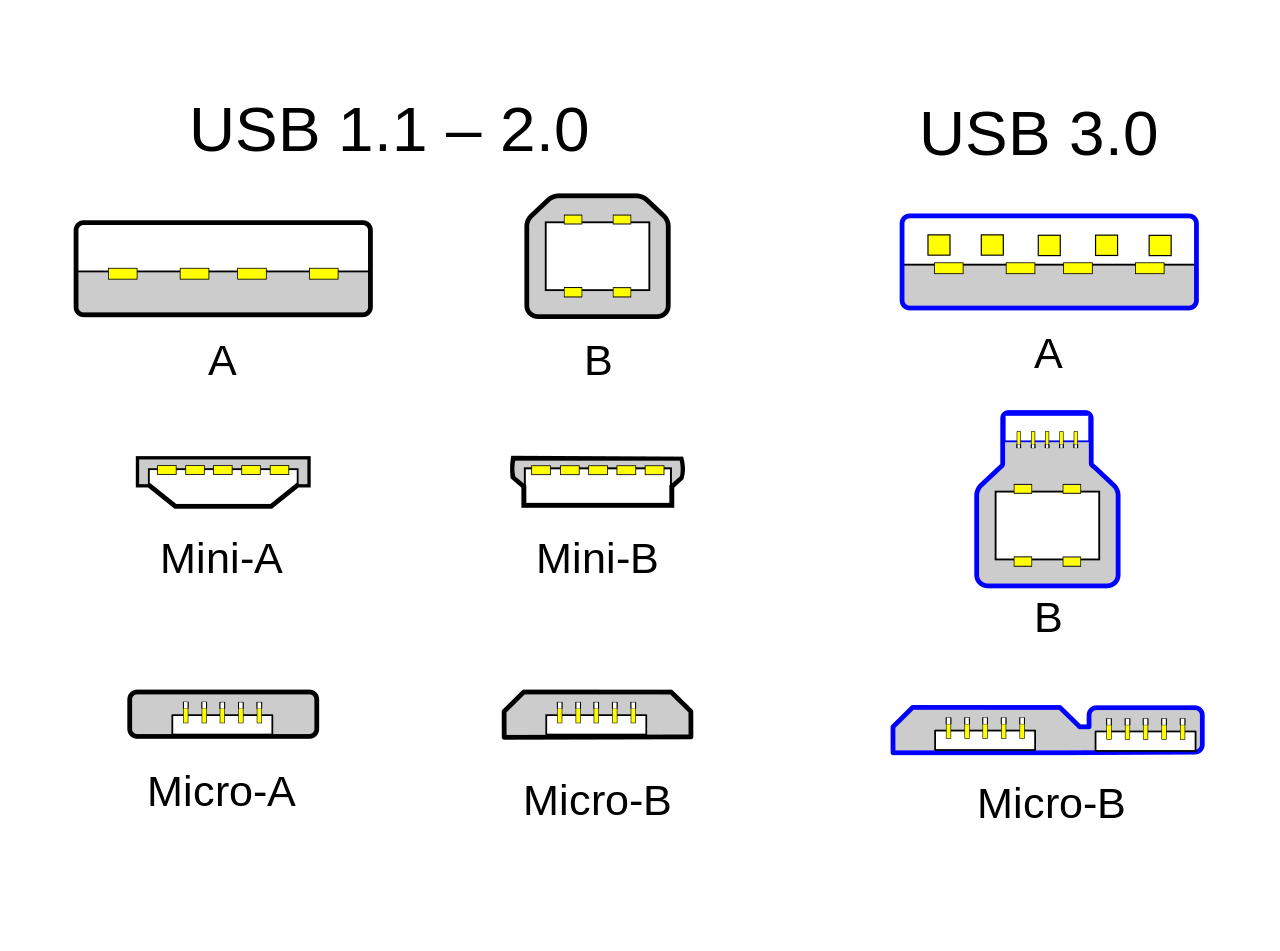
\includegraphics[width=0.4\textwidth]{images/usb_connectors.png}
    \caption{Connectors USB de tipus A i B. \cite{Contributors2024USB}}
    \label{fig:usb_connectors}
\end{figure}

\begin{itemize}
    \item Els connectors de tiups A son els que es connecten al dispositiu
    que actuarà com a mestre. Existeixen les variants \est{micro} i \est{mini},
    com es pot observar a la Figura \ref{fig:usb_connectors}, tot i que aquestes
    so son gaire populars. Amb l'aparició de l'estàndard \acro{usb3}, es van
    dissenyar nous connectors que fóssin compatibles amb els dels estàndards
    anteriors.
    \item Els connectors de tipus B son els que es connecten a l'esclau. Aquests
    també tenen les variants \est{micro} i \est{mini}, molt utilitzades
    en l'electrònica domèstica. També es va crear nous connectors de tipus B
    per a poder acollir l'estàndard \acro{usb3}.
    \item Finalment, els connectors de tipus C no tenen una jerarquia definida:
    serveixen per a dispositius que poden ser mestres o esclaus en diferents
    moments donats. La decisió de qui actua de mestre es pacta just a l'inici
    de la connexió, mitjançant un protocol específic \cite{Axelson2015USB}.
    Aquest connector, a diferència de la reta, és reversible: es pot connectar
    en les dues orientacions possibles. Es pot veure l'aspecte del connector
    a la Figura \ref{fig:usb_connectors_c}.
\end{itemize}

\begin{figure}[ht]
    \centering
    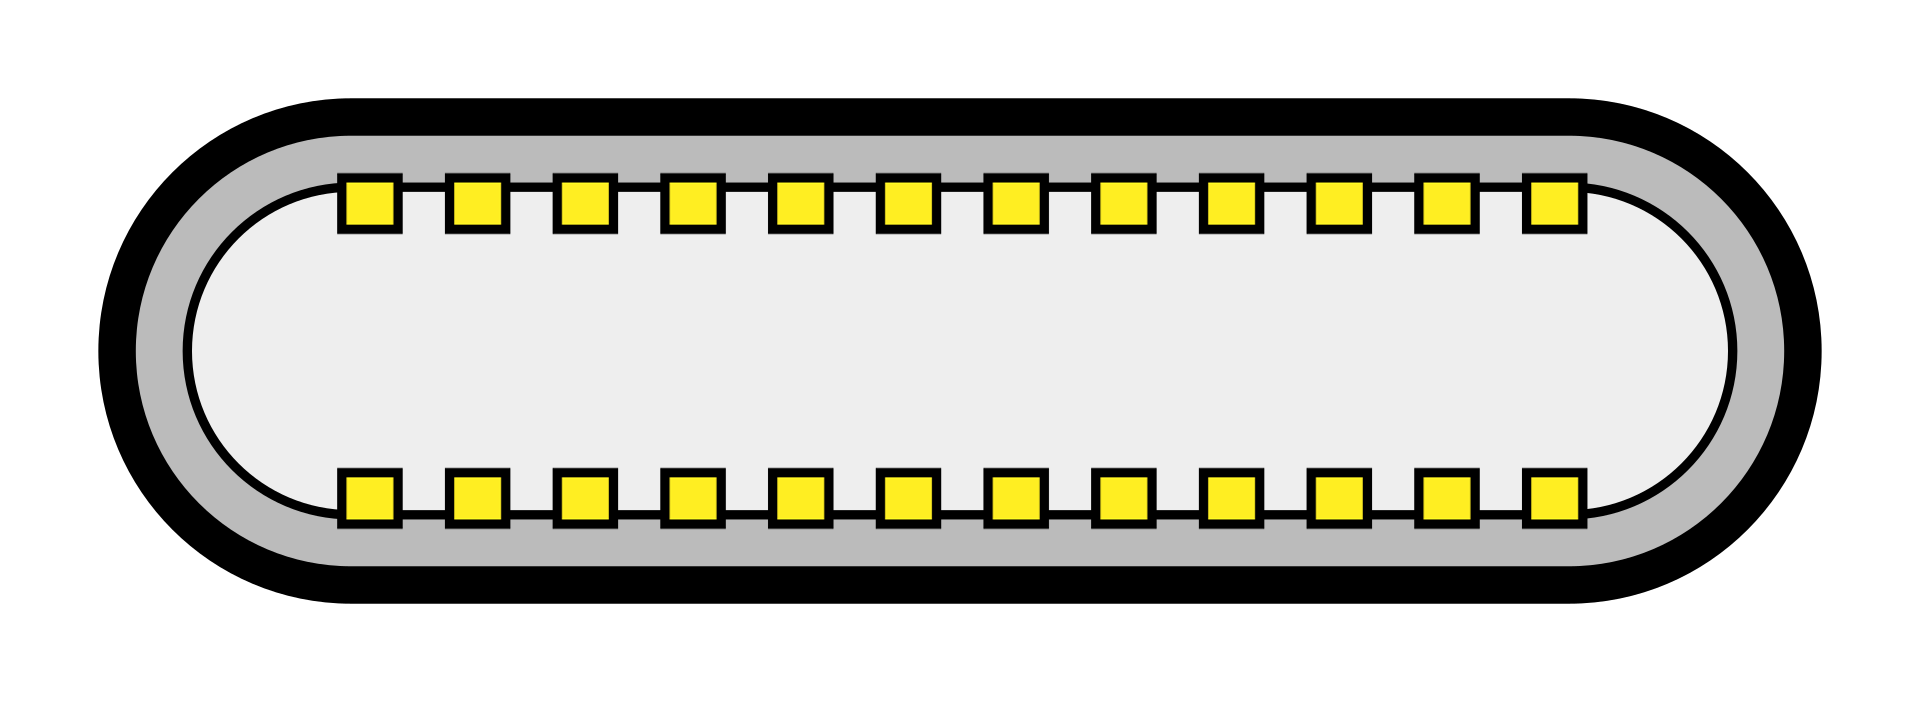
\includegraphics[width=0.2\textwidth]{images/usb_c.png}
    \caption{Connector USB de tipus C. \cite{Contributors2024USB}}
    \label{fig:usb_connectors_c}
\end{figure}

Així doncs, gairebé la totalitat de cables \acro{usb} seran de tipus A a tipus
B, utilitzant qualsevol format de mida. El tipus C, al ser bidireccional, pot
substituir el tipus A o el tipus B en els cables mencionats anteriorment.
Quan un cable només té un connector de tipus C en un cantó, no s'ha de pactar
la jerarquia de mestre-esclau, ja que ve definida pel tipus de connector a
l'altra banda del cable. Evidentment, també hi pot haver cables de tipus C a
tipus C.

Tanmateix, a l'any 2022 el Consell de la Unió Europea va aprovar una llei
que obliga un seguit de dispositius electrònics a utilitzar el connector
\acro{usb-c} enlloc d'altres estàndards \cite{Council2022Common}. Segons la
nota de premsa, el motiu d'aquesta llei és per a evitar més deixalla electrònica
per culpa de tenir diferents dispositius amb diferents connectors, així com
facilitar l'ús de les tecnologies als consumidors. Aquesta llei
es començarà a aplicar a finals de l'any 2024, i afectarà dispositius mòbils, 
alguns portàtils, tauletes, teclats i ratolins ina\l.làmbrics, entre
d'altres.

Sent el dispositu que es vol crear en aquest projecte un perifèric de
l'ordinador, la llei citada no l'afectaria. Tanmateix, la mateixa nota de premsa
informa sobre la intenció d'extendre aquest connector a altres dispositius.
Tenint present que el dispositiu que es vol crear podria entrar fàcilment en
aquest grup de perifèrics d'ordinador, s'ha decidit utilitzar un connector de
tipus \acro{usb-c} per a assegurar-nos la seva possible comercialització dintre
de la \acro{UE}.

\section{Taules d'ús \acro{hid}}
\label{sec:hut}

Tal i com s'ha comentat en l'apartat \ref{subsubsec:metadades}, els dispositius
\acro{hid} utilitzen uns protocols ja establerts per a poder ser utilitzats
sense haver d'insta\l.lar programari nou a l'ordinador (el que es coneix com
a \est{plug\&play}).

Un cop es presenta un dispositiu com a \acro{hid}
(mitjançant les metadades), s'ha d'enviar a l'ordinador una nova capçalera de
metadades, donant més informació sobre el dispositiu. Aquest paquet s'anomena
\est{\acro{Hid} Report Descriptor} i envia informacions molt detallades de
quin dispositiu és i com envia les dades.

Per exemple, un ratolí definirà que cada poc temps l'ordinador podrà fer-li
una petició de noves dades, i que aquestes tindran el format de 3 valors
de 1 bit (pels 3 botons), i 2 valors de 8 bits (per a saber la disància
desplaçada en cadascún dels eixos de coordenades). Aquesta capçalera també
especificarà que el dispositiu és un ratolí. Un cop enviat aquest paquet,
l'ordinador ja sabrà com comunicar-se amb el
dispositiu i com interpretar les dades que anirà enviant.

La documentació oficial de \acro{usb} \cite{HidHut} especifica
detalladament tots els codis que es poden definir. El que interessarà per a
aquest treball és la categoria de \textit{Sensors}, i dintre d'aquesta hi ha
diversos tipus de dispositius. Veurem que el tipus \est{3D Accelerometer} serà
el més adequat per al projecte.

Aquesta documentació anterior es pot complementar amb una guia d'interpretació
de la documentació de Linux \cite{LinuxHid} on es presenten diferents eines
per a interpretar millor aquests paquets. Tot i que n'hi ha moltes que
funcionen des del terminal, la més visual i popular és \est{wireshark}.

Un dels altres avantatges d'utilitzar \acro{hid} és que, al ser una capa per
sobre del protocol \acro{usb}, és independent d'aquest. En altres paraules,
altres protocols de comunicació poden beneficiar-se també de \acro{hid}, no
només \acro{usb}. Per aquest motiu, quan es va implementar \est{Bluetooth},
es va decidir utilitzar també \acro{hid} \cite{BluetoothHid}.

\subsection{Acceleròmetre tridimensional}

Tal i com es veurà més endavant, s'acabarà utilitzant la categoria de
\est{3D Accelerometer} per a designar el tipus de dispositiu. Aquesta
categoria (i la resta de dispositius dins del subgrup de sensors) necessita
reportar un seguit de dades, i no totes són òbvies.

A continuació es detallen les diferents dades que s'ha d'enviar. Tal i com s'ha
comentat anteriorment, en el \est{\acro{hid} report descriptor} es definirà
el tipus de dispositiu i el format i valors de les dades que s'enviarà, juntament
amb la freqüència amb que l'ordinador les pot so\l.licitar.

\begin{itemize}
    \item En primer lloc, s'ha de comunicar el tipus exacte de dispositiu. En
    aquest cas, la categoria de sensors i el tipus acceleròmetre tridimensional.
    \item S'ha de comunicar el tipus de connexió amb l'ordinador: integrat a
    la mateixa màquina, extern o adjunt. En el cas d'aquest projecte s'utilitzarà
    el tipus \textit{adjunt}, ja que es troba a molta proximitat de l'ordinador
    i reportarà dades del mateix (el tipus extern seria per a sensors que
    mesuren variables d'altres aparells).
    \item També s'ha de reportar els esdeveniments que pugui tenir el sensor.
    En aquest cas, no hi ha events a reportar, així que en aquest paquet
    es definirà solament el tipus genèric \est{No Events}.
    \item L'estat d'alimentació del dispositiu també serà constant per a
    aquest dispositiu (no s'implementarà mode \est{sleep} o de baix consum, i
    la diferència de consum mentre que s'agafen mostres i mentre que
    s'espera una nova lectura de dades és poc significatiu). Tanmateix, el
    protocol també ordena enviar-ho de la mateixa forma que la resta d'estats.
    \item El següent valor a enviar és l'estat del sensor. Aquest sí que serà
    diferent en funció de les dades que reporti el sensor. Per exemple, pot
    reportar que hi ha noves dades, que s'està inicialitzant, que hi ha un
    error en la lectura de dades, entre d'altres.
    \item Es reportarà també l'interval que proposa el dispositiu entre
    diferents \est{reports}, és a dir, el temps que separarà cada trama de
    tipus \acro{in}.
    \item Finalment, hi ha les dades que es vol enviar. En la capçalera inicial
    s'especificarà moltes configuracions referent a les dades: valor màxim,
    mínim, factor d'escala, estat de les dades. Es recomana llegir la
    documentació proposada o veure exemples per a entendre la immensitat
    d'aquesta informació.
\end{itemize}

Un cop enviada aquesta capçalera,
l'ordinador podrà demanar tantes vegades com vulgui els valors de les dades.
Concretament, en el cas d'aquest sensor, l'ordinador podrà demanar dos tipus
de dades: \est{feature} i \est{input}.

\begin{itemize}
    \item El tipus \est{feature} enviarà l'estat del sensor: connexió, dades,
    intèrval entre comunicacions, sensitivitat i esdeveniments.
    \item El tipus \est{input} enviarà l'estat del sensor i, si s'escau, els
    valors llegits. Aquests valors s'hauran de dividir pel factor especificat
    a la capçalera per a poder representar decimals. En el cas de l'acceleròmetre,
    l'unitat a enviar és \textit{g}, i poques vegades aquest valor superarà mai
    les poques unitats, pel que disposar de decimals és essencial.
\end{itemize}

La tasca a efectuar quan es dissenyi el programari serà convertir la
informació anterior en el format desitjat per al protocol \acro{hid}. Per sort,
existeixen programes i eines que ajuden a generar aquests codis, tal i com
es veurà més endavant.

\section{V-USB}

Una de les eines que facilita la implementació del protocol \acro{usb} és la
llibreria \acro{v-usb}, implementada per \est{Objective Development}
\cite{Vusb}. Aquesta llibreria
es distribueix amb la llicència \acro{gpl-2+}, una llicència que obliga a
distribuir sota la mateixa llicència (o versions posteriors d'aquesta) tots els
projectes que facin servir la llibreria. La empresa ofreix el concecpte de
llicència dual: a part de \acro{gpl-2+}, es pot comprar una llicència comercial
per a poder generar codi sota altres llicències \cite{VusbLicensing}.

Aquesta llibreria implementa la capa més baixa de \acro{usb} a l'arquitectura
\acro{avr}, sense utilitzar perifèrics específics. Així doncs, gràcies a aquesta
llibreria no serà necessari utilitzar un microcontrolador \acro{avr} dotat amb
perifèrics \acro{usb}, com podria ser, per exemple l'\acro{AtMega32u4}.

La probabilitat d'acabar utilitzant un microcontrolador \acro{avr} per a aquest
projecte és molt elevada, degut a la prèvia experiència personal amb aquesta
arquitectura. També hi ha gran varietat d'exemples i llibreries disponibles per
a \acro{avr}, cosa que facilitarà la tasca de desenvolupament.

A \cite{Vusb} hi ha el codi font de la llibreria, que s'ha d'incloure al
projecte que s'estigui desenvolupant, i també s'hi troben exemples de dispositius
senzills (ratolins i teclats) implementats amb aquesta llibreria. Tanmateix,
s'ha trobat el repositori de \cite{VusbProjects} més interessant, ja que conté
exemples de sensors \acro{hid}.

\section{\est{Drivers} a Linux}

Un altre dels aspectes importants del projecte és la creació d'un programari
que pugui fer d'intermediari entre el dispositiu i l'entorn gràfic. Tal i com
diu el títol de l'apartat, es comentarà només el cas específic dels sistemes
\acro{UNIX}, concretament amb Linux.

El \est{kernel} de Linux acostuma a dividir tot en diferents capes, i no és una
excepció per al que té referència amb aquest projecte. Sempre és recomanable
treballar amb la capa més alta possible, ja que sovint aixó significa
estalviar-se feina. Tanmateix, és important comprendre d'on es vé per a
poder entendre millor els errors i dificultats que es trobaran en aquest treball.

\subsection{Permisos: \acro{udev}}

\acro{Udev} és un gestor de dispositius per a sistemes basats en Linux.
Té com a objectiu gestionar dinàmicament els dispositius de maquinari del
sistema, és a dir, és el responsable que si es connecta o desconnecta
un dispositiu mentre l'ordinador està encès tot funcioni amb normalitat \cite{Udev}.

El funcionament d'\acro{udev} es basa en un conjunt de regles,
que es configuren per
determinar com han de gestionar-se els dispositius detectats.
Aquestes regles es poden configurar i modificar, i en el cas d'aquest projecte
s'utilitzaran exclusivament per a permetre a tots els usuaris utilitzar alguns
dispositius concrets, siguin quins siguin els permisos. Tanmateix, \acro{udev}
ofereix molta flexibilitat: es poden executar \est{scripts}, canviar el nom,
crear un volum, entre moltes altres possibilitats.

Com és d'esperar, només un usuari amb permisos d'administrador podrà configurar
les regles \acro{udev}, i hi ha molts paràmetres per a configurar al màxim
aquestes regles. Tanmateix, com que aquestes normes només seran d'utilitat durant
el procés de desenvolupament del dispositiu, s'ha decidit no entrar gaire en
detalls de la implementació.

\subsection{Capa 1: \acro{libusb}}

\est{libusb} és una llibreria multiplataforma i disponible per diversos
llenguatges que permet realitzar una comunicació amb dispositius \acro{usb} en
la capa més baixa possible. En aquest nivell es poden enviar trames de control,
entrada o sortida a nivell de bits i bytes \cite{Libusb}.

Tot i que la llibreria es va pensar
incialment per Linux, s'ha portat a Windows i MacOS, convertint-la en la millor
alternativa per a generar programes multiplataforma que necessitin controladors
personalitzats.

Tanmatix, aquest projecte es beneficiarà de les capes de més alt nivell, pel que
serà més fàcil utilitzar les altres llibreries, tot i que això pugui suposar
efectuar petits canvis entre els diferents sistemes operatius.

A Linux, un dispositiu que es pot controlar per \est{libusb} sol aparéixer com
a fitxer sota el format \verb|/dev/usbrawX|, on X és el número de dispositiu.
No gens menys, si un contro\l.lador d'una capa superior està utilitzant
exclusivament el dispositiu, el \est{kernel} no crearà aquest fitxer, per a
evitar confusió i so\l.lapaments.

\subsection{Capa 2: \acro{libhid} i \acro{hidapi}}

La següent llibreria és la capa immediatament superior a la de l'apartat
anterior. \est{libhid} permet gestionar dispositius \acro{hid}. D'questa
llibreria ha nascut \est{hidapi}, que la engloba i la converteix en
una abstracció compatibla amb altres sistemes operatius, com
FreeBSD, Windows i MacOS \cite{Libhid}. Tal i com s'ha dit a 
l'apartat \ref{sec:hut}, també permetrà utilitzar dispositius Bluetooth.

Al ser aquesta llibreria una abstracció més elevada, existeixen més aplicacions
per a provar-la i debugar-la. Sobretot es destaca \cite{LibhidUI}, que disposa
d'una interfície molt senzilla d'utilitzar i multiplataforma.

A Linux, un dispositiu que es pot controlar per \est{libhid} sol aparéixer com
a fitxer sota el format \verb|/dev/hidrawX|, on X és el número de dispositiu.
De la mateixa forma que amb l'apartat anterior, el dispositiu no apareixerà
sota aquest format si una capa més alta l'està utilitzant exclusivament.

\subsection{Capa 3: \acro{libiio}}

Finalment, la darrera capa d'abstracció de la pila d'aquest projecte és la
llibreria \acro{libiio}.
Aquesta llibreria permet interaccionar amb el sistema
\acro{iio} de Linux. També està disponible per a diversos llenguatges, però
a diferència de la resta d'abstraccions, no és multiplataforma.

El sistema \acro{iio}, o \est{Industrial Input/Output}, és la capa d'abstracció
dels sistemes basats en Linux per a qualsevol dispositiu que suposi una entrada
o sortida per al sistema i no tingui contro\l.ladors dedicats. Per exemple, un
ratolí o teclat no entraria en aquest grup, ja que disposa de controladors
propis \cite{Iio}.

Hi ha moltes formes de veure quines categories de dispositius \acro{hid} es
converteixen en \acro{iio}, però la més senzilla és consultant el codi
font de Linux \cite{KernelIioAccel}. Pel que fa a aquest projecte, es pot veure
que esisteix un \est{driver} per a \est{hid\_accelerometer\_3d}, pel que
el dispositiu d'aquest treball anirà en aquesta capa superior.

Mitjançant normes \acro{udev} es podria aconseguir que un dispositiu que, per 
defecte s'assigna a \acro{iio} es quedi una capa més per sota, com seria
\acro{hid} o \acro{usb}. Tanmateix, \acro{iio} aporta molts beneficis.

\begin{itemize}
    \item No necessita permisos suplementaris per a llegir les dades dels
    sensors. Per tant, no s'ha d'afegir a l'usuari en un grup nou ni crear
    cap regla \acro{udev}.
    \item Més d'un usuari o procés pot estar llegint simultàniament el sensor.
    El dispositu creat a \verb|/dev/iio:deviceX| (on X és el número de
    dispositiu) pot ser llegit simultàniament, de la mateixa forma que ho fan
    altres fitxers, per exemple \verb|/dev/rand| o \verb|/dev/zero|.
    \item Al ser una capa superior, no s'ha de gestionar tot el referent al
    protocol \acro{hid}. Les lectures del sensor venen gairebé completament
    processades.
    \item Finalment, al ser una capa superior, també hi tene cabuda altres
    sensors que podrien servir per al projecte, però que no són \acro{hid}.
\end{itemize}

Així doncs, es pagarà el preu de generar programari no compatible amb altres
dispositius a canvi de generar programari robust i a la capa més alta possible
per Linux. Pot semblar una mala decisió, però es veurà en el següent apartat
que tampoc seria possible generar un controlador 100\% multiplataforma.

\subsection{Serveis: \est{systemd}}
\label{subsec:systemd}

El programari que es pretén realitzar per a aquest projecte involucra la
presència d'un procés que, en tot moment, comprovi les lectures del sensor i
actualitzi l'orientació de la pantalla. L'usuari és responsable d'insta\l.lar i
configurar el programa, però un cop configurat, aquest hauria de funcionar
correctament sempre, fins i tot després de reiniciar l'ordinador.

En els sistemes basats en Linux, els programes que estan en execució tota
l'estona s'anomenen serveis i els gestiona el propi \est{kernel}, també anomenat
en aquest context \est{systemd} \cite{Systemd}. Hi ha dos tipus de serveis diferents, en
funció dels privilegis que tenen:

\begin{itemize}
    \item Els \textit{serveis del sistema} afecten a tots els usuaris i
    s'executen sota l'usuari i context de \est{root} (excepte si es diu
    el contrari). Es pot escollir quan s'executen, ja sigui just després de
    carregar el \est{kernel} a la memòria o després que el primer usuari
    inicii sessió. Es necessiten permisos d'administrador per a fer modificacions
    en els serveis de sistema (generalment mitjançant la comanda
    \verb|systemctl|).
    \item Els \textit{serveis d'usuari}, en canvi, només afecten a l'usurari
    que els ha configurat. No es necessiten permisos d'administrador per a
    configurar-los, i s'executen sota el mateix context, variables d'entorn i
    usuari que qui els ha configurat. Aquests serveis només es poden executar a
    partir dels darrers passos de l'arrencada del sistema, ja sigui després
    d'iniciar sessió o un cop carregat l'entorn gràfic. També utilitzen la
    comanda \verb|systemctl|, però afegint l'opció \verb|--user|.
\end{itemize}

És important conéixer la diferència entre els dos tipus mencionats, ja que en
aquest treball es generarà un servei d'usuari i un de sistema, i cadascún té
les seves complicacions, tant en el moment d'insta\l.lació com en el moment
d'execució.

\subsection{Entorn gràfic: \acro{Xlib}}

Finalment, un cop es sap com es farà la lectura de les dades del sensor, cal
esbrinar com s'aplicarà els canvis de rotació de la pantalla. Els sistemes
basats en Linux, independentment de l'entorn gràfic que utilitzin (normalment
\acro{gnome}, però també \acro{kde}), responen a les peticions gràfiques sota
l'interfície de programació de \est{Xlib} \cite{Xlib}.

Es podria fer una bona analogia entre
els entorns gràfics i els navegadors: els navegadors, a Linux, implementen les
crides i interfície de \est{www-browser}, tot i estar implementats internament
de formes diferents. Si es vol implementar una aplicació que necessiti, per
exemple, un navegador incrustat, però qualsevol navegador serveix, es pot
indicar com a dependència \est{www-browser} enlloc de, per exmple, \est{firefox}.

\est{Xlib} és una llibreria molt complexa, i té interfícies per a la majoria
de llenguatges. Tanmateix, sovint és més senzill utilitzar una aplicació de
la línia de comandes que simplifica la tasca del programador. Aquesta
aplicació és diu \est{xrandr}, i d'una forma molt senzilla permet llistar
totes les pantalles connectades a l'ordinador i canviar l'orientació
d'una d'elles \cite{Xrandr}. Ara bé, els beneficis venen amb un cost: les sessions.

\subsection{\est{Xrandr} i les sessions}
\label{subsec:xrandr}

Els sistemes Linux estan construits per a ser el més versàtils possible. Una
de les possibilitats és que hi hagi diferents clients connectats a la vegada
a la mateixa màquina. Aquest fet no sorprèn a ningú, ja que és ben sabut que
diversos usuaris poden connectar-se remotament i simultàniament a la mateixa
màquina mitjançant \est{ssh}. Ara bé, hi ha diverses formes (com, per exemple,
la opció \verb|-X| de \est{ssh}) que permeten diferents sessions gràfiques
simultàniament \cite{ManSSH}.

La complicació rau en que \est{xrandr} utilitza les variables d'entorn per a
trobar la sessió actual. Aquestes variables es defineixen a l'inici de sessió,
quan s'inicialitza \est{Xlib}. Això vol dir que, sempre que s'executi
\est{xrandr} des de la sessió (ja sigui amb un servei de sessió o a través de
la línia de comandes) no hi haurà problema.
Tanmateix, si es vol executar \est{xrandr} des d'un servei de sistema o d'un
terminal remot, el programa no trobarà la sessió actual i serà impossible
resoldre la comanda.

Hi ha entre dos i tres variables d'entorn importants per al correcte funcionament
de \est{xrandr} \cite{XrandrVars}:

\begin{itemize}
    \item La variable d'entorn \verb|$DISPLAY| permet identificar el grup de
    pantalles al que s'està connectat. En general sermpre serà \verb|:0| (o 
    \verb|:1| pels sistemes més recents), però si hi ha diversos usuaris
    connectats amb diferents entorns gràfics podria ser un altre nombre.
    \item La segona variable d'entorn necessària és \verb|$XAUTHORITY|. Aquesta
    variable conté la direcció del fitxer \est{Xauthority}. Aquest fitxer
    conté la \est{cookie} que permet consultar i realitzar canvis en la sessió
    actual. Com és evident, aquest fitxer només es pot consultar per l'usuari
    propietari de la sessió (i usuaris administradors).
    \item Finalment hi ha \verb|$XDG_RUNTIME_DIR|, que preten reemplaçar la
    variable anterior per a portar la direcció del directori que conté el fitxer
    \est{Xauthority}.
\end{itemize}

Cal tenir present que un usuari pot restringir qui té accés a modificar la
seva sessió. Per defecte, es restringeix a tothom que no tingui accés al
fitxer d'autorització, però mitjançant la comanda \verb|xhost +| es pot permetre
que tothom pugui efectuar modificacions a la sessió d'aquell usuari \cite{xhost}.
Tanmateix, es considera aquesta pràctica poc segura, i per aquest motiu no es
tindrà en compte durant l'elaboració d'aquest treball.

\subsection{\est{Wayland}}
\label{subsec:wayland}

El servidor gràfic de l'apartat anterior, \est{Xorg}, és un projecte molt vell
i porta acumulades bastantes funcionalitats i canvis que s'ha fet durant els
anys. Si bé és molt funcional i popular, es podria crear un entorn gràfic que
funcionés d'una forma més eficient amb el maquinari actual (el \est{harrdware}
ha canviat molt des dels seus inicis). Aquesta és la idea que va tenir les
persones que van impulsar \est{Wayland}.

Creat a l'any 2008, ha anat recuperant totes les funcionalitats de \est{Xorg}
implementades amb una arquitectura bastant diferent. Tot i seguir sent
compatible amb alguns aspectes senzills, hi ha molts programes que deixen de
funcionar amb aquest nou servidor, especialment els que comparteixen pantalla
o interactuen amb ella. Des de Ubuntu 17.10 que el sistema operatiu deixa
escollir entre els dos entorns \cite{Wayland}.

Tanmateix, un canvi d'aquesta embargadura no es fa d'una versió per una altra.
\est{Wayland} encara necessita bastantes millores per a fer-lo completament
compatible, pel que la seva \acro{api} no és del tot definitiva. Es preveuen
encara uns anys fins que no s'anuncii la data en la que \est{Xorg} haurà de
ser utilitzat. I un cop passada aquesta data el més probable és que comandes
com \verb|xrandr| segueixin funcionant, de la mateixa forma que segueixen
funcionant eines com \verb|ifconfig|, deprecades des de fa ja molts anys
\cite{Ifconfig}.

Per aquest motiu s'ha decidit realitzar el projecte utilitzant \est{Xorg}.
D'aquesta forma s'obtindrà un programari estable, si més no durant els primers
anys. Així doncs, si el projecte té previsió de continuar més enllà d'aquest
Treball de Fi de Grau s'haurà de preveure una migració a \est{Wayland}.
